\newpage
\chapter{Проектирование}
Выше были выделены основные компоненты системы и разграничены функции и
ответственность между ними. Теперь необходимо определиться с конкретной
реализацией выбранных компонентов и со схемой взаимодействия между ними. Так же
необходимо спроектировать даталогическую модель базы данных. При выборе
реализации необходимо учитывать требования к системе в целом.

\section{Общая архитектура системы }
\begin{figure}[h]
\center{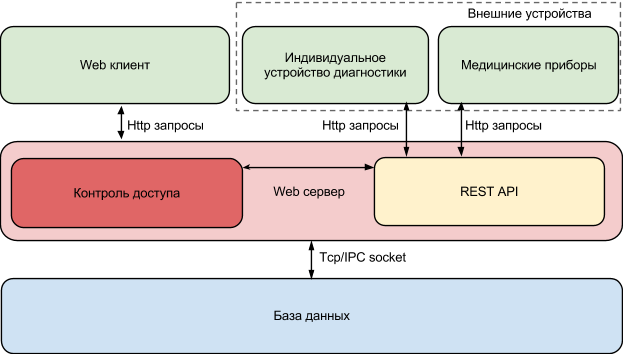
\includegraphics[width=1\linewidth]{general_architecture.eps}}
\caption{Общая архитектура системы.}
\label{ris:general_architecture}
\end{figure}

На рисунке \ref{ris:general_architecture} изображено